%!TEX root = 16-ra-letter-NMPCWalkGen.tex
\section{Dynamic Filter}
\label{Sec:dynamic_filter}
%
%In \cite{herdt:iros:2010}, the authors apply $T=100$ms and a preview window containing $N=16$ samples, i.e.~$T\cdot N=1.6$s.
%This horizon corresponds to two foot steps.

\begin{figure}[h]
  \begin{center}  
    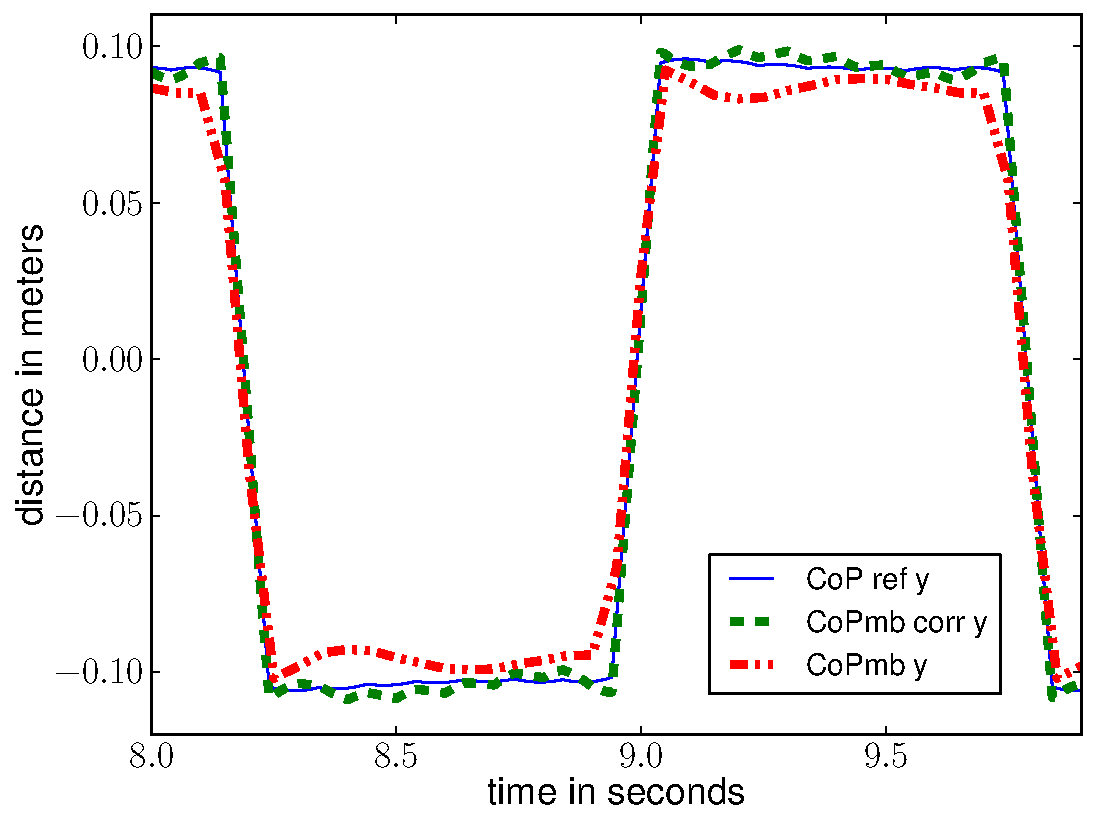
\includegraphics[width=0.8\linewidth]{./copmby.pdf}
    \caption[CoP filtered]{
      Result of the dynamic filtering on the CoP.
      In solid blue, the reference CoP computed by the solver.
      In dash-dot-dot red, the CoP multi-body.
      In dashed green, the CoP multi-body recomputed after correction.
    	}
    \label{fig:resultDynamicFilter}
  \end{center}
\end{figure}

Recall that the algorithm presented in this chapter and the one presented in \cite{herdt:iros:2010} assume that the inertial effect of the legs and the arms are neglected.
An interesting fact is that the algorithm in \cite{herdt:iros:2010} that was successfully implemented on the \mbox{HRP-2} in the Japan Robotic Laboratory (JRL),
turned out to be unstable for its first test on another \mbox{HRP-2} robot located at LAAS-CNRS.
In order to cope with this difficulty, we used the dynamic filter introduced by Kajita \cite{Kajita:icra:2003}.
This filter aims to correct the difference between the referenced CoP computed by the pattern generator and the CoP reconstructed from 
the joint trajectories finally realized on the robot.
In order to do so, a second model predictive control is used.
This technique is often seen as applying a Newton Raphson method on the following equation
$ z^{ref}(t) = RNEA(q (t)),$
where $RNEA$ is the Recursive Newton-Euler Algorithm applied on the multi-body robot model. 
It computes the multi-body CoP from
$q$, the generalized spatial state vector at time $t$.
In general this method does not guarantee the convergence, and might suffer from numerical instability.
However, it has proven its efficiency for this specific problem \cite{Nishiwaki2007}.
Indeed in practice one iteration of the dynamic filter is sufficient to reduce considerably the error on the CoP (see Fig.~\ref{fig:resultDynamicFilter}).
More technical details about this algorithm are shown in Annexe~\ref{an:dyn:filter}.

\section{Experiments with \mbox{HRP-2}}
\label{sec:experiments_with_hrp2}

\newcommand{\widthValue}{0.30\linewidth}
\begin{figure}[h]
  \begin{center}
  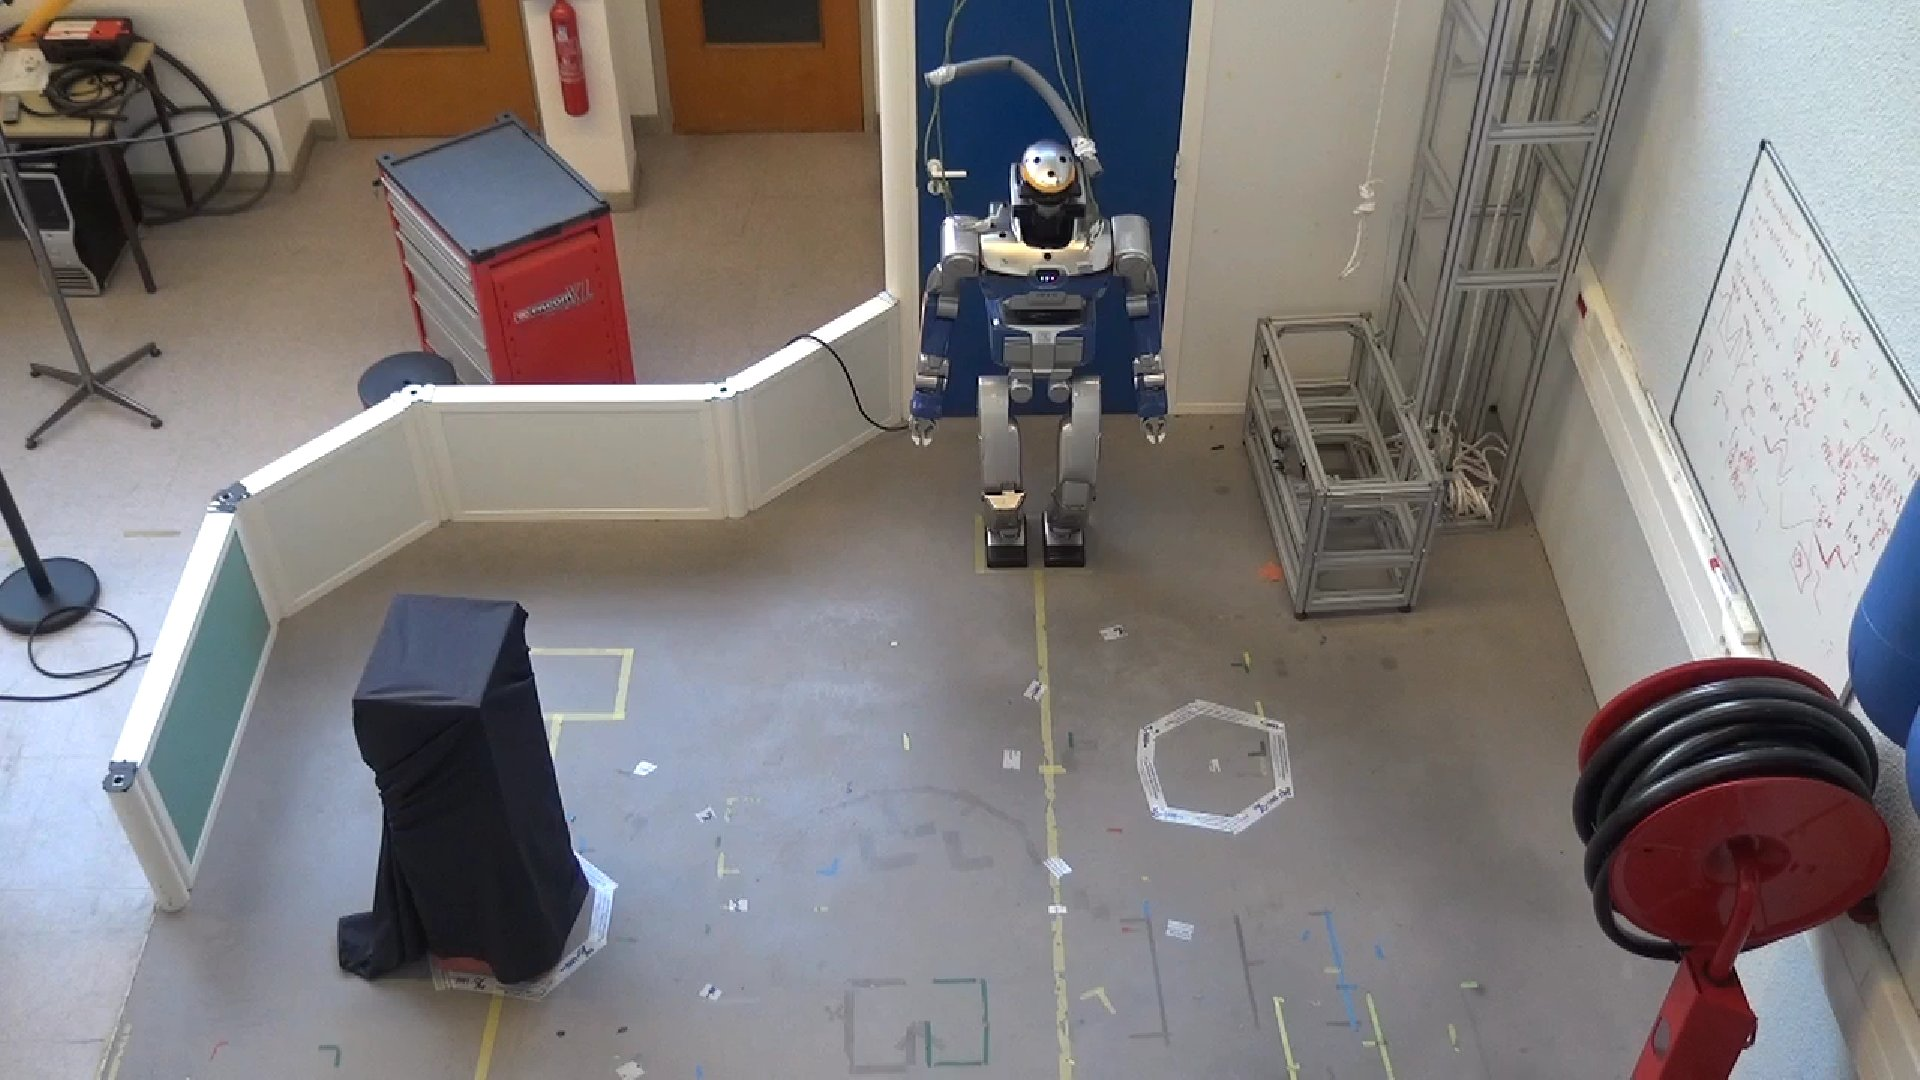
\includegraphics[trim={10.0cm 0.0cm 17.0cm 0.0cm}, clip, width=\widthValue]
    {./pictures_from_movie/top_view1.jpeg}
  \includegraphics[trim={10.0cm 0.0cm 17.0cm 0.0cm}, clip, width=\widthValue]
    {./pictures_from_movie/top_view2.jpeg}
  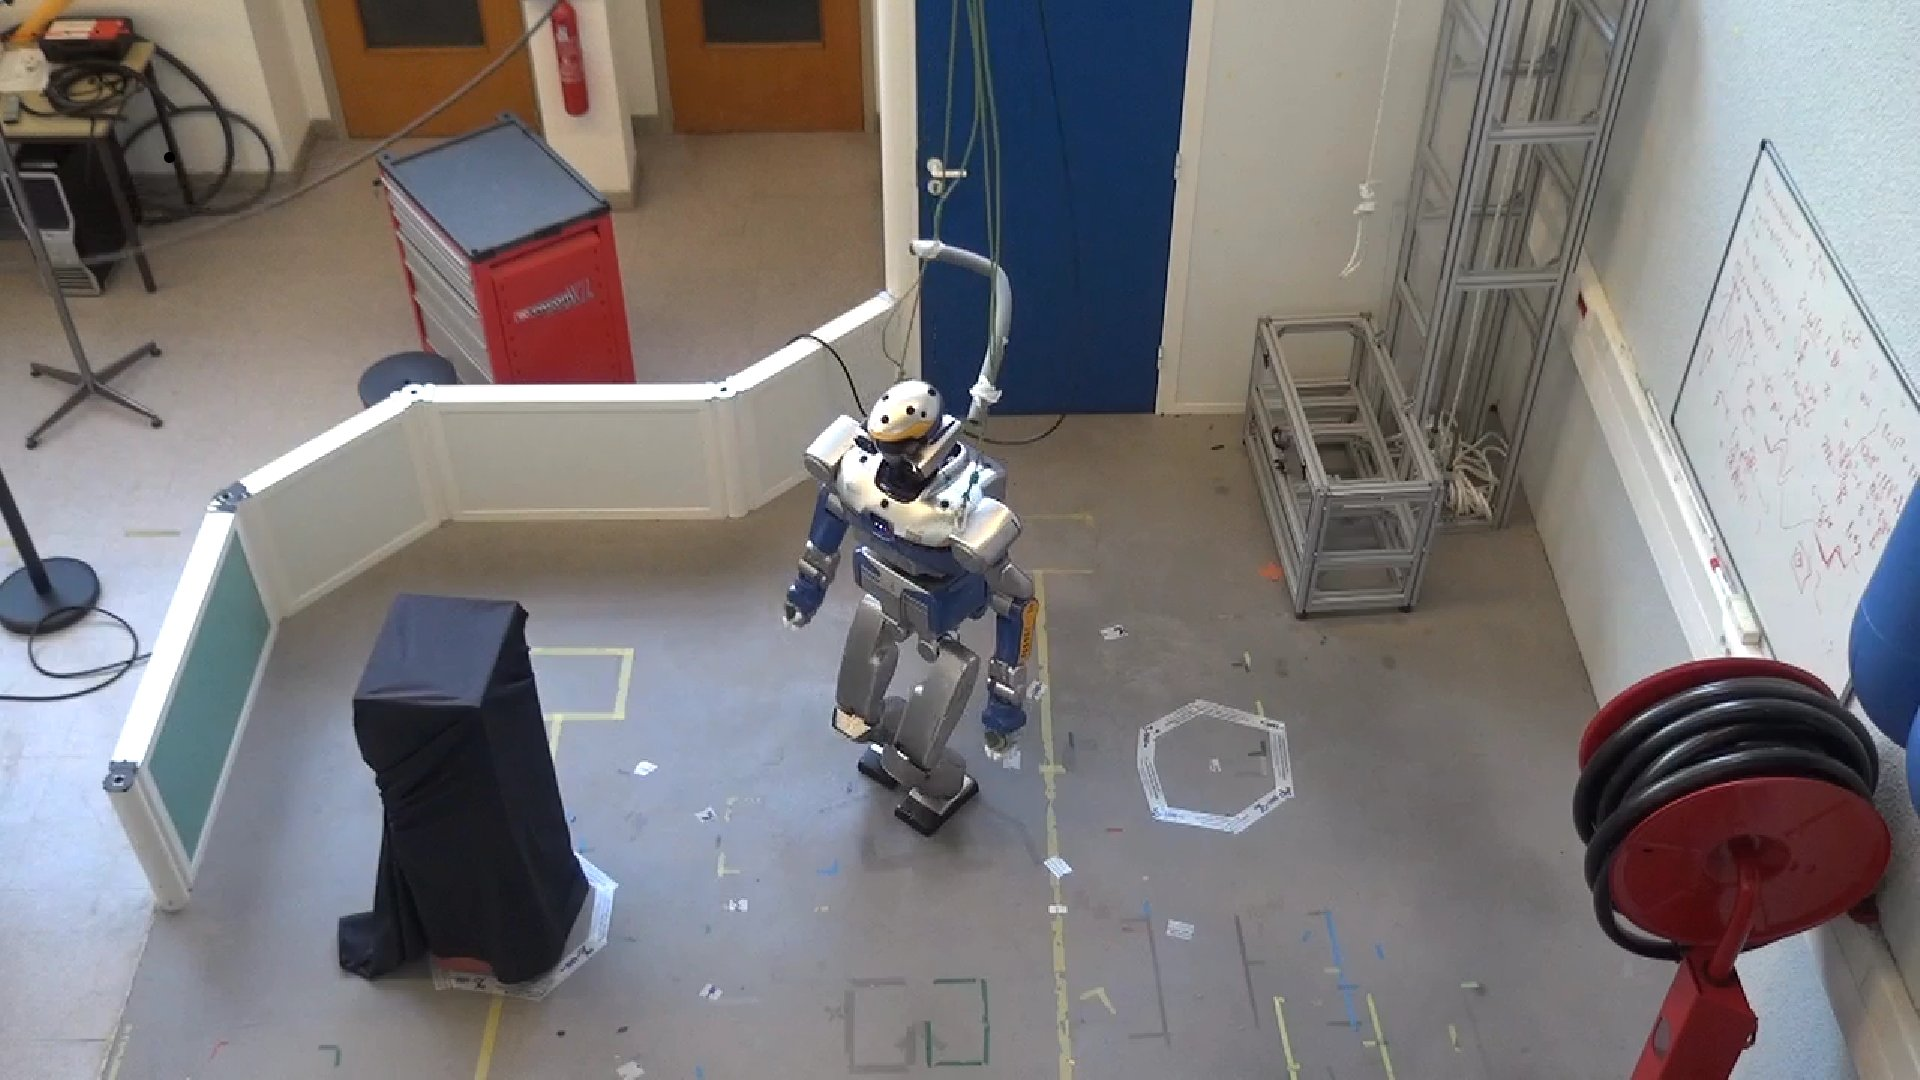
\includegraphics[trim={10.0cm 0.0cm 17.0cm 0.0cm}, clip, width=\widthValue]
    {./pictures_from_movie/top_view3.jpeg}
  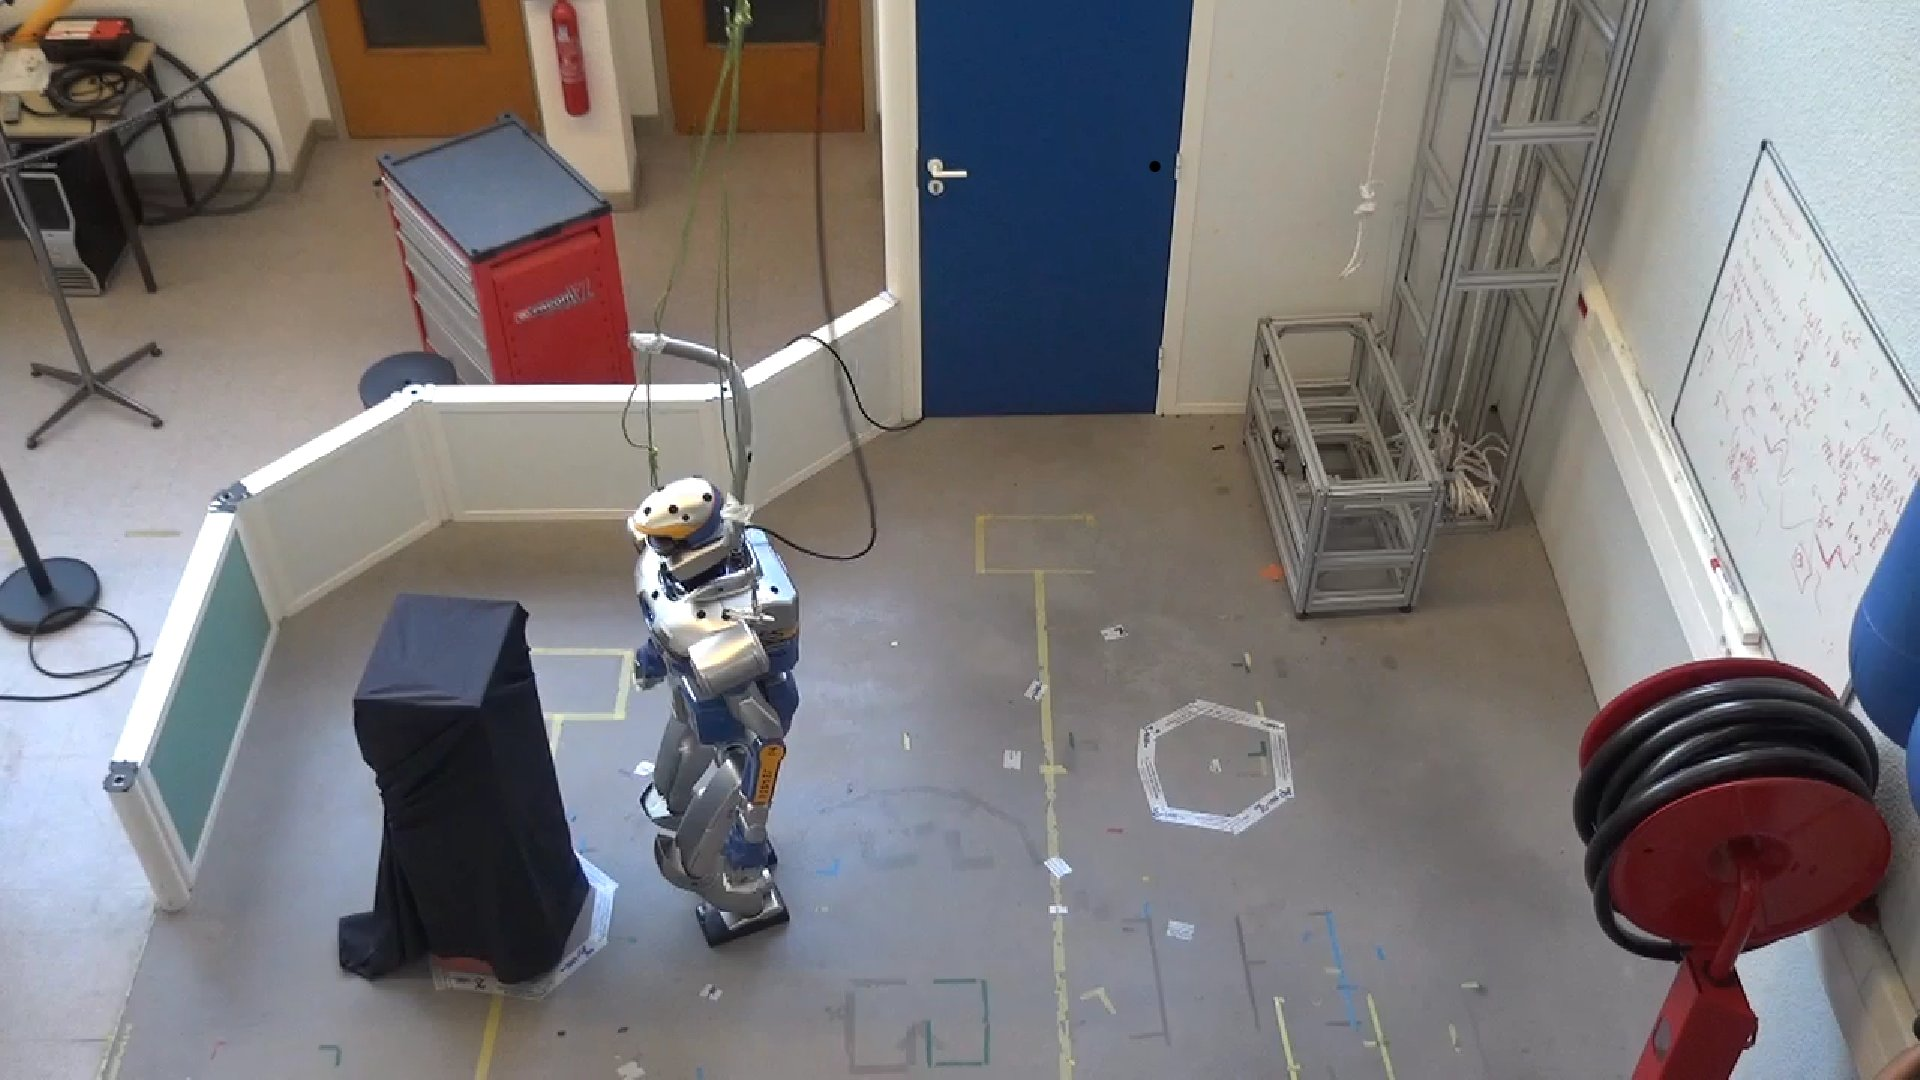
\includegraphics[trim={10.0cm 0.0cm 17.0cm 0.0cm}, clip, width=\widthValue]
    {./pictures_from_movie/top_view4.jpeg}
  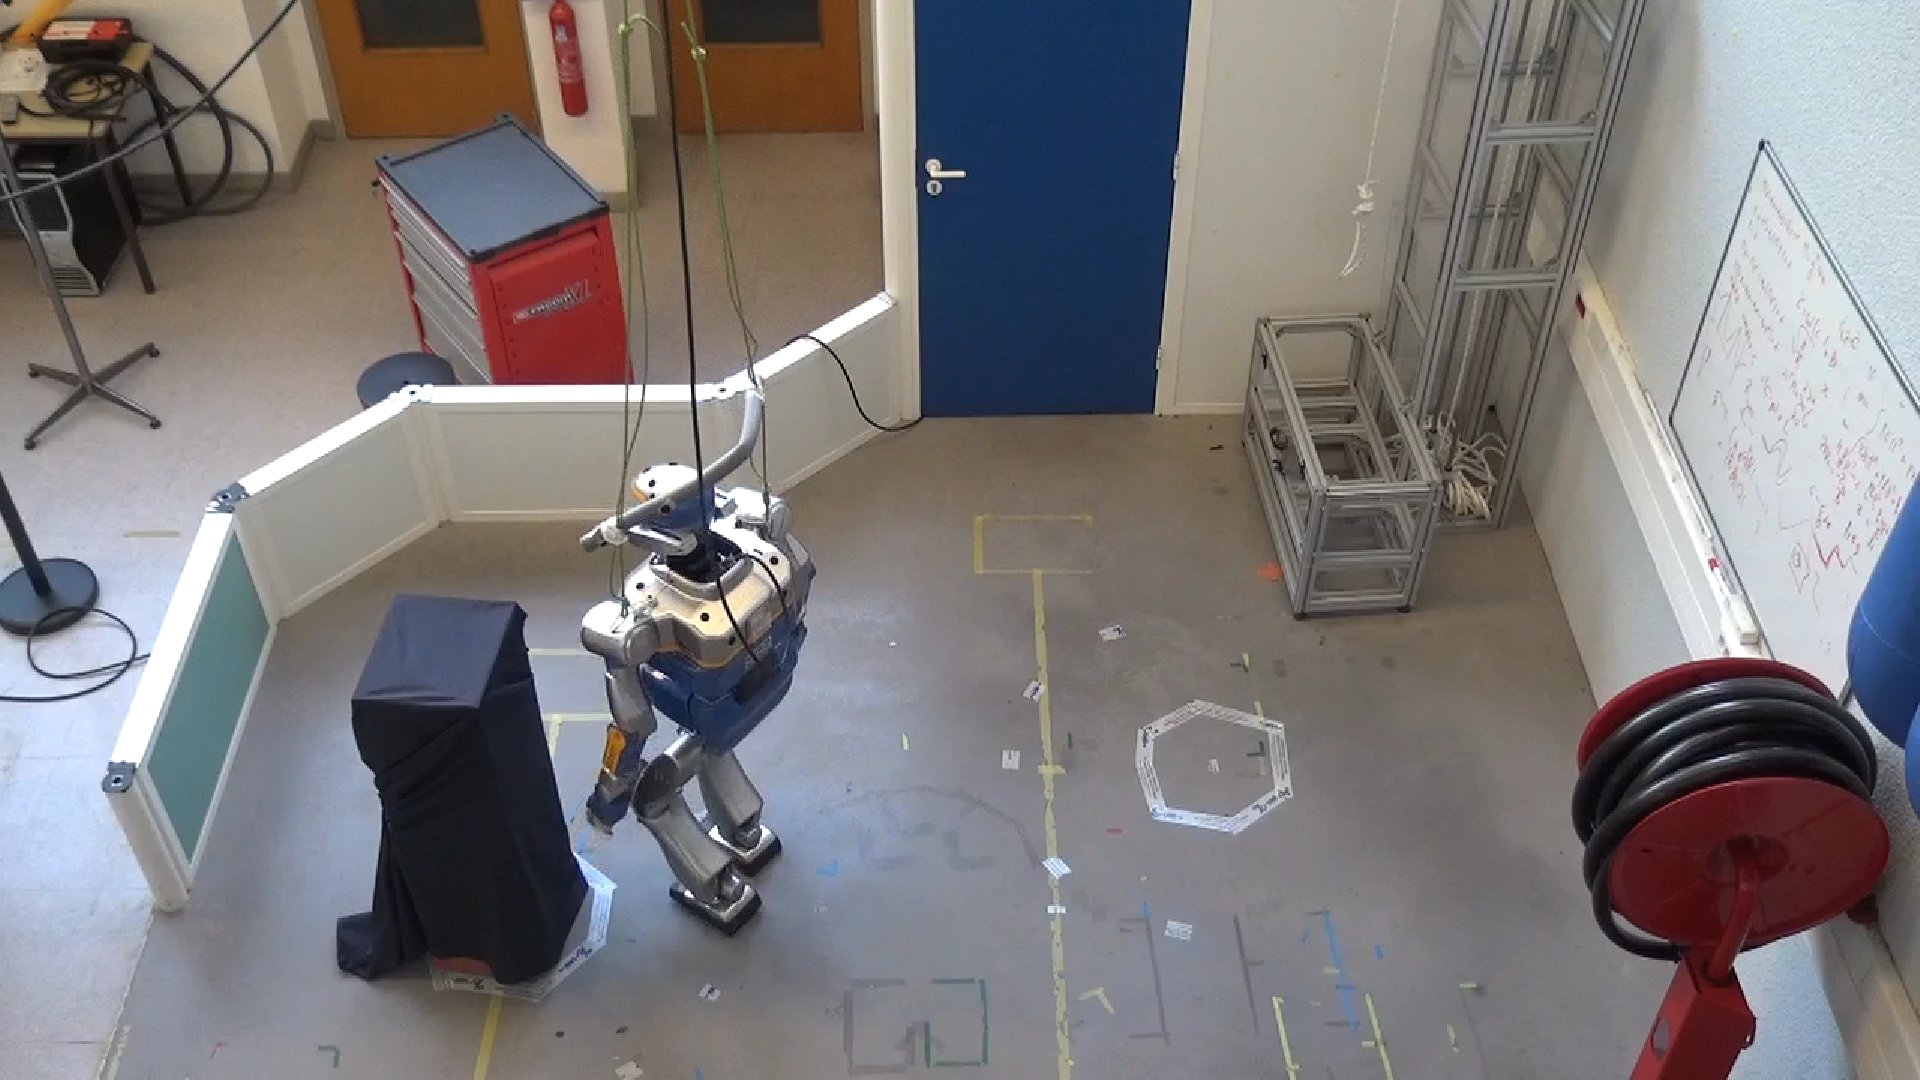
\includegraphics[trim={10.0cm 0.0cm 17.0cm 0.0cm}, clip, width=\widthValue]
    {./pictures_from_movie/top_view5.jpeg}
  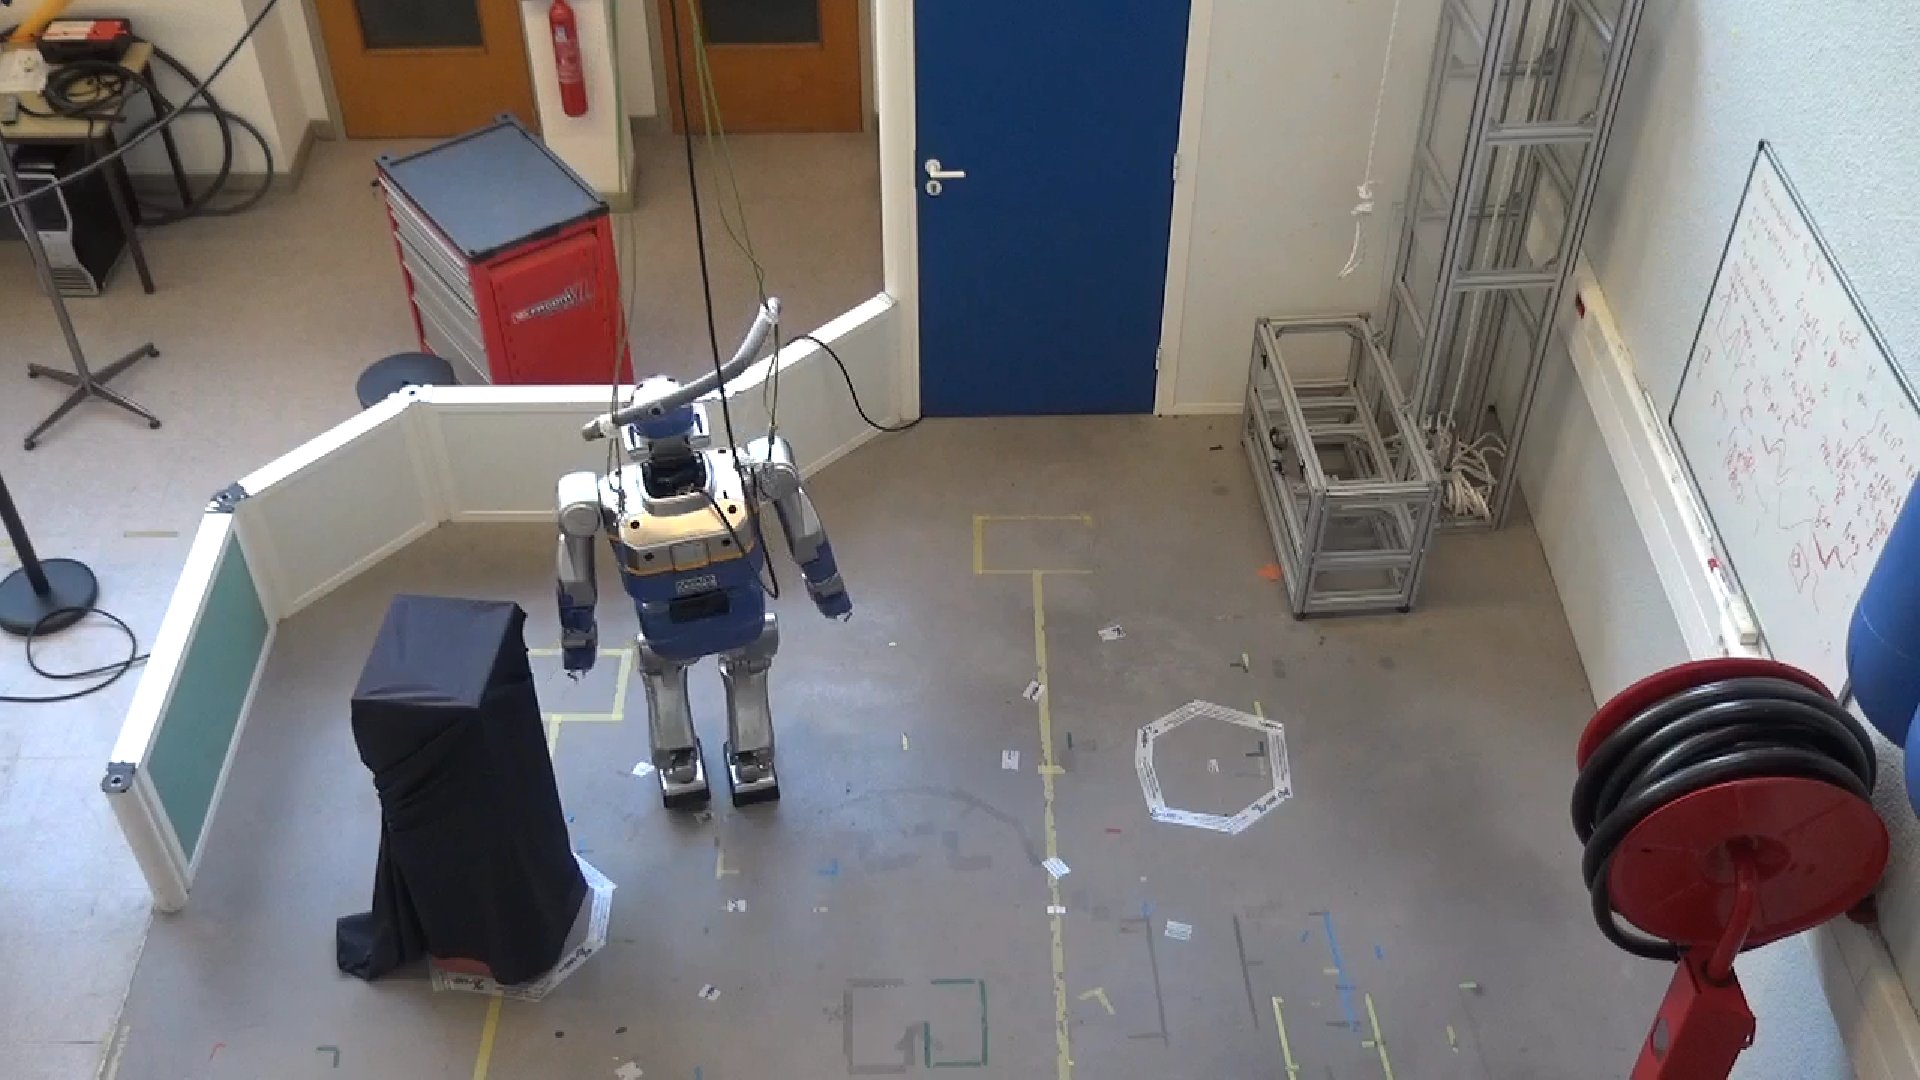
\includegraphics[trim={10.0cm 0.0cm 17.0cm 0.0cm}, clip, width=\widthValue]
    {./pictures_from_movie/top_view6.jpeg}
    %trim={<left> <lower> <right> <upper>}
  \caption{
    Experiment on the HRP-2 robot using the setup B.
  }
  \label{fig:hrp2_experiment}
  \end{center}
\end{figure}
%Descente de newton raphson : equivalent a une iteration du ddp de Mujoco,
%-> introduction du corps complet, suffisant pour compenser la majeur partie des effets dynamique

In this section two experiments on the \mbox{HRP-2} humanoid robot are presented.
As described in the introduction they correspond to local situations where a foot-step planner using a discrete set of foot-step transitions may fail.
We consider the case where only a reference velocity is given to drive the robot.
It corresponds to a sensor-based behavior such as the one presented in \cite{garcia:ijrr:2015}.
The integration with a reactive planner such as the one presented \cite{perrin:itro:12} is left for future work.
In the first experiment, the reference velocity drives the robot towards an obstacle which can be avoided thanks to the WPG.
The second experiment shows the robot performing a circular trajectory and avoiding an obstacle.

\subsection{Experimental setup}

The duration of one full step is $0.8\,s$, including single support ($0.7\,s$) and double support ($T=0.1s$).
During the experiment the preview horizon of the NMPC is two full steps, while the preview horizon of the dynamic filter is equal to one full step 
in order to insure real time feasibility on \mbox{HRP-2}.\\
Fig.~\ref{fig:trajectories} depicts the two experimental setups.
The upper figure and Fig.~\ref{fig:covernmpcwalkgen} show the output of the algorithm in the situation \emph{A}.
The forward velocity is set to ${Vel}_{k+1}^{ref}$~$=$~$[0.2,0,0]$ and the obstacle to avoid is the red box.
In Fig.~\ref{fig:trajectories} the box is represented by the inner red circle while the security margin is represented by the outer green circle.
The robot is allowed to step on the green circle but not inside it.
This margin prevents the upper body from colliding with the obstacle.
%\fbox
\begin{figure}[h]
  \begin{center}
    \subfloat[Situation~\emph{A}]{
      \fbox{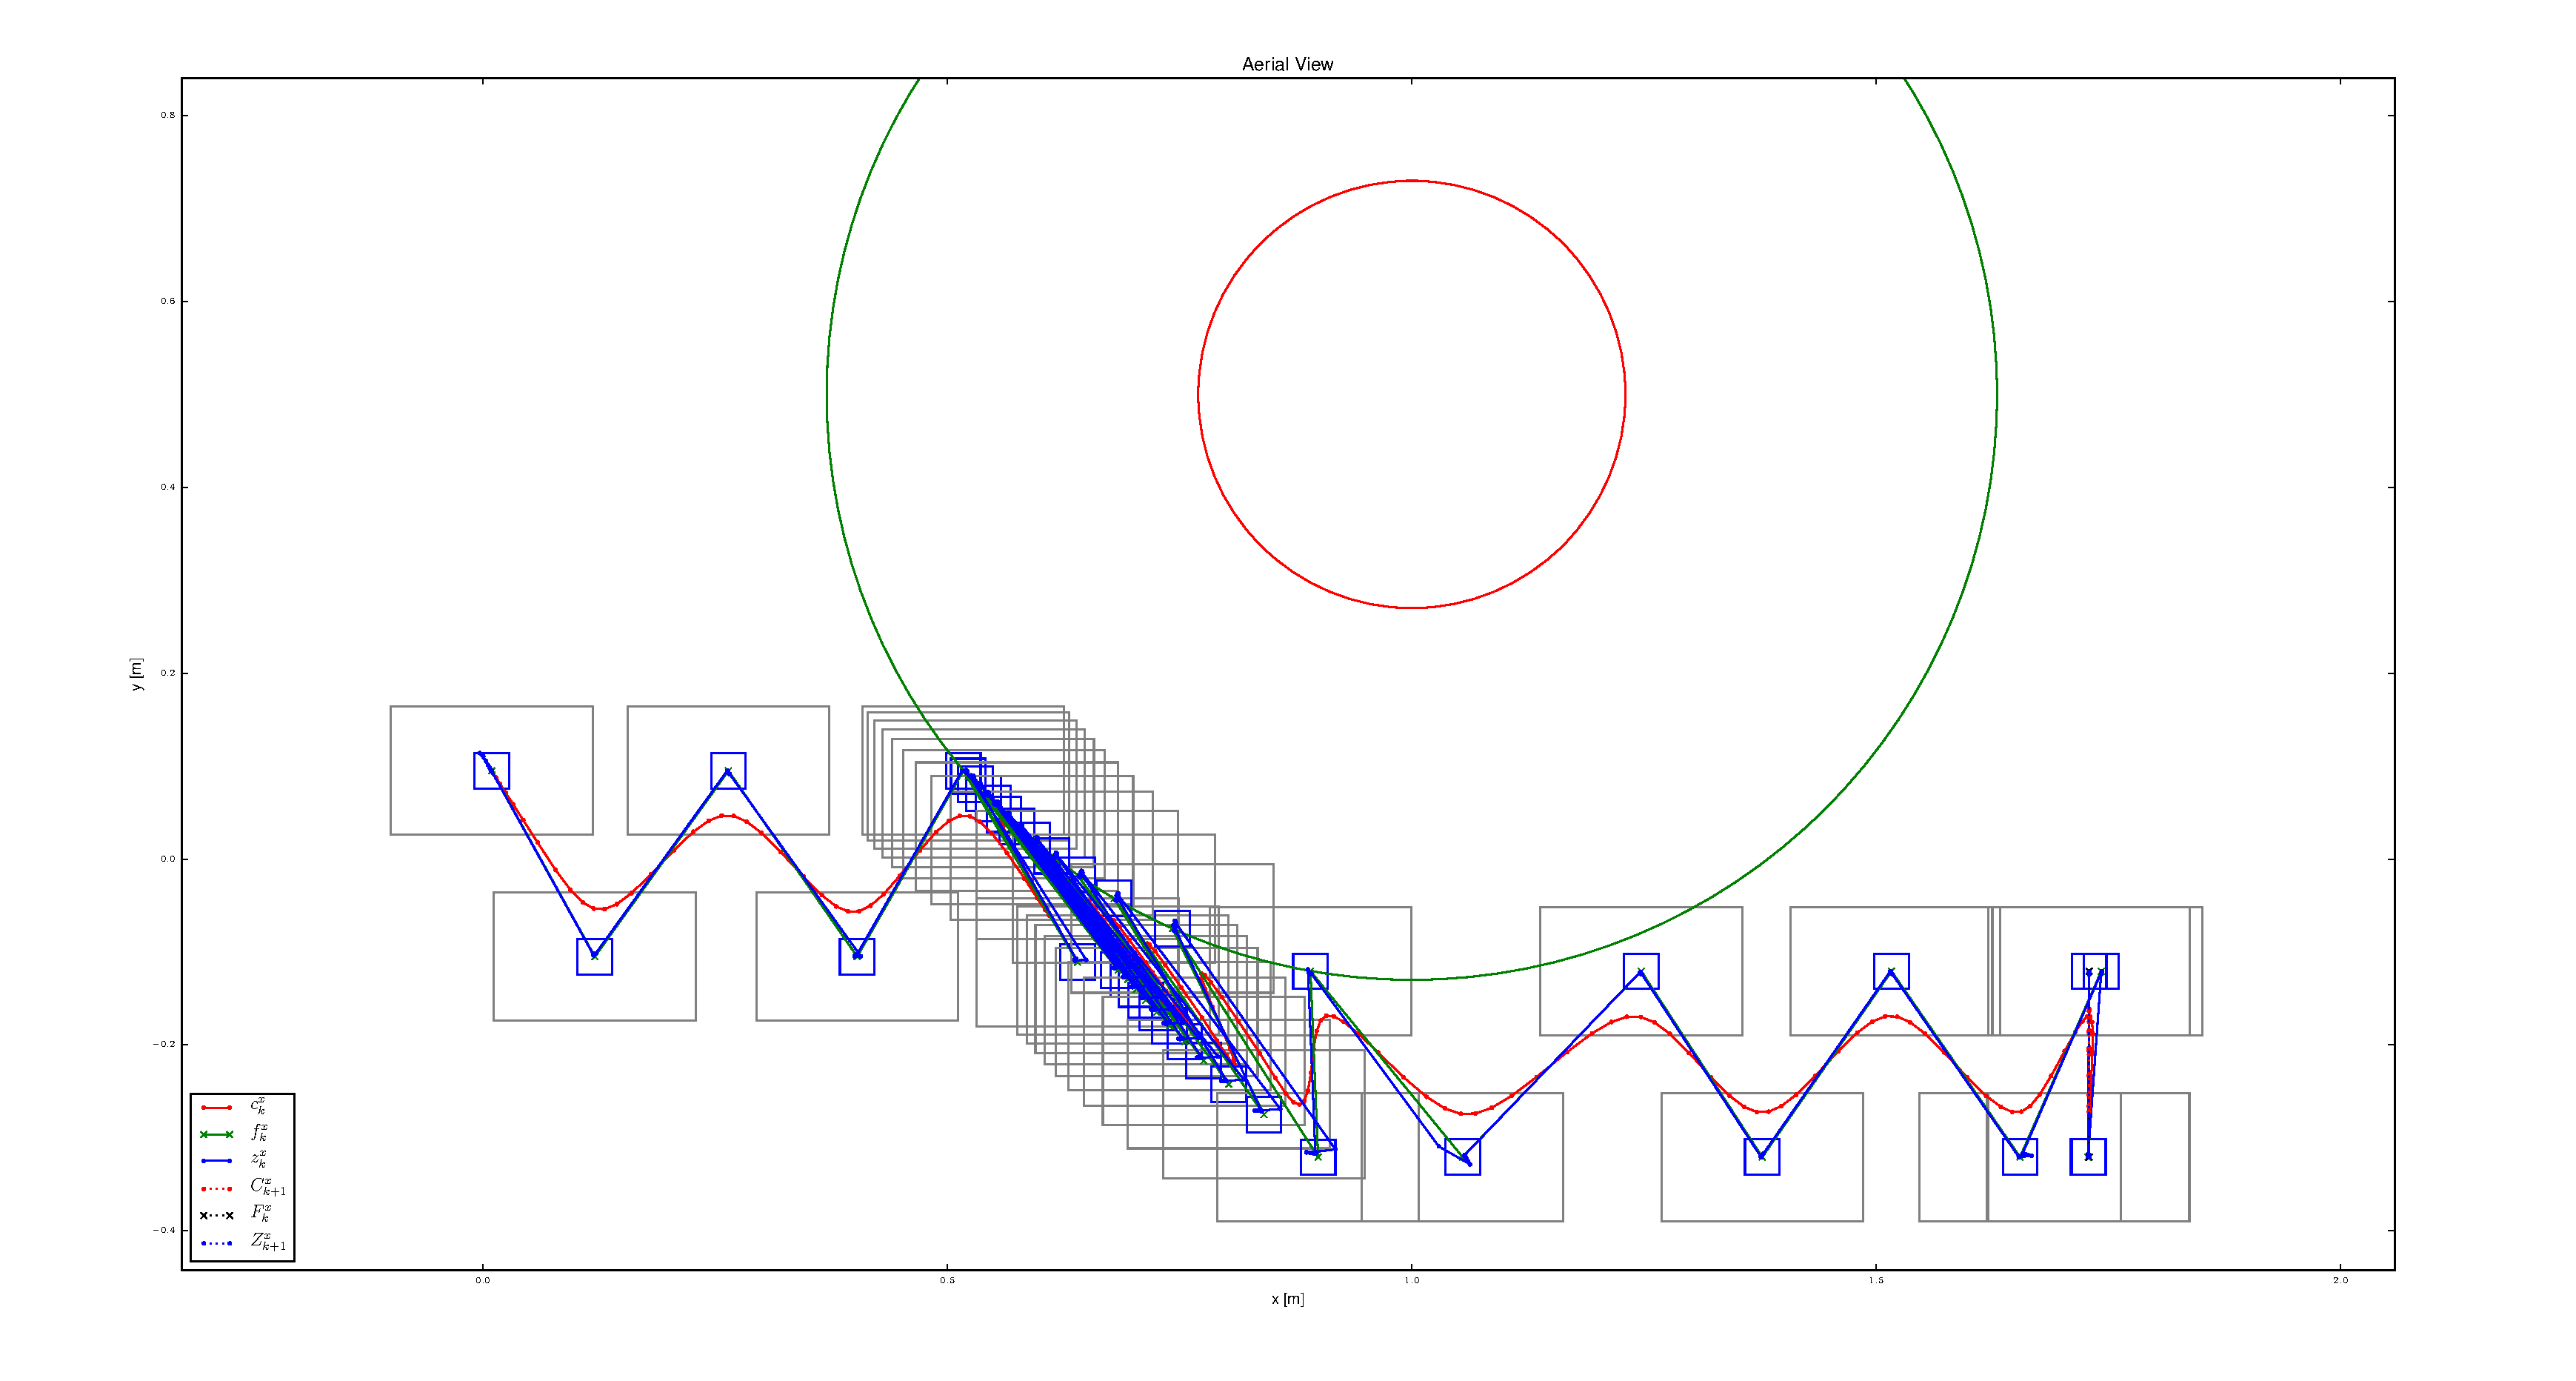
\includegraphics[trim={8.0cm 3.0cm 8.0cm 2.0cm},
        clip, width=0.45\linewidth]{./setupA.pdf}}
      \label{subfig:trajectoriesB}
    }
    \subfloat[Situation~\emph{B}]{
      \fbox{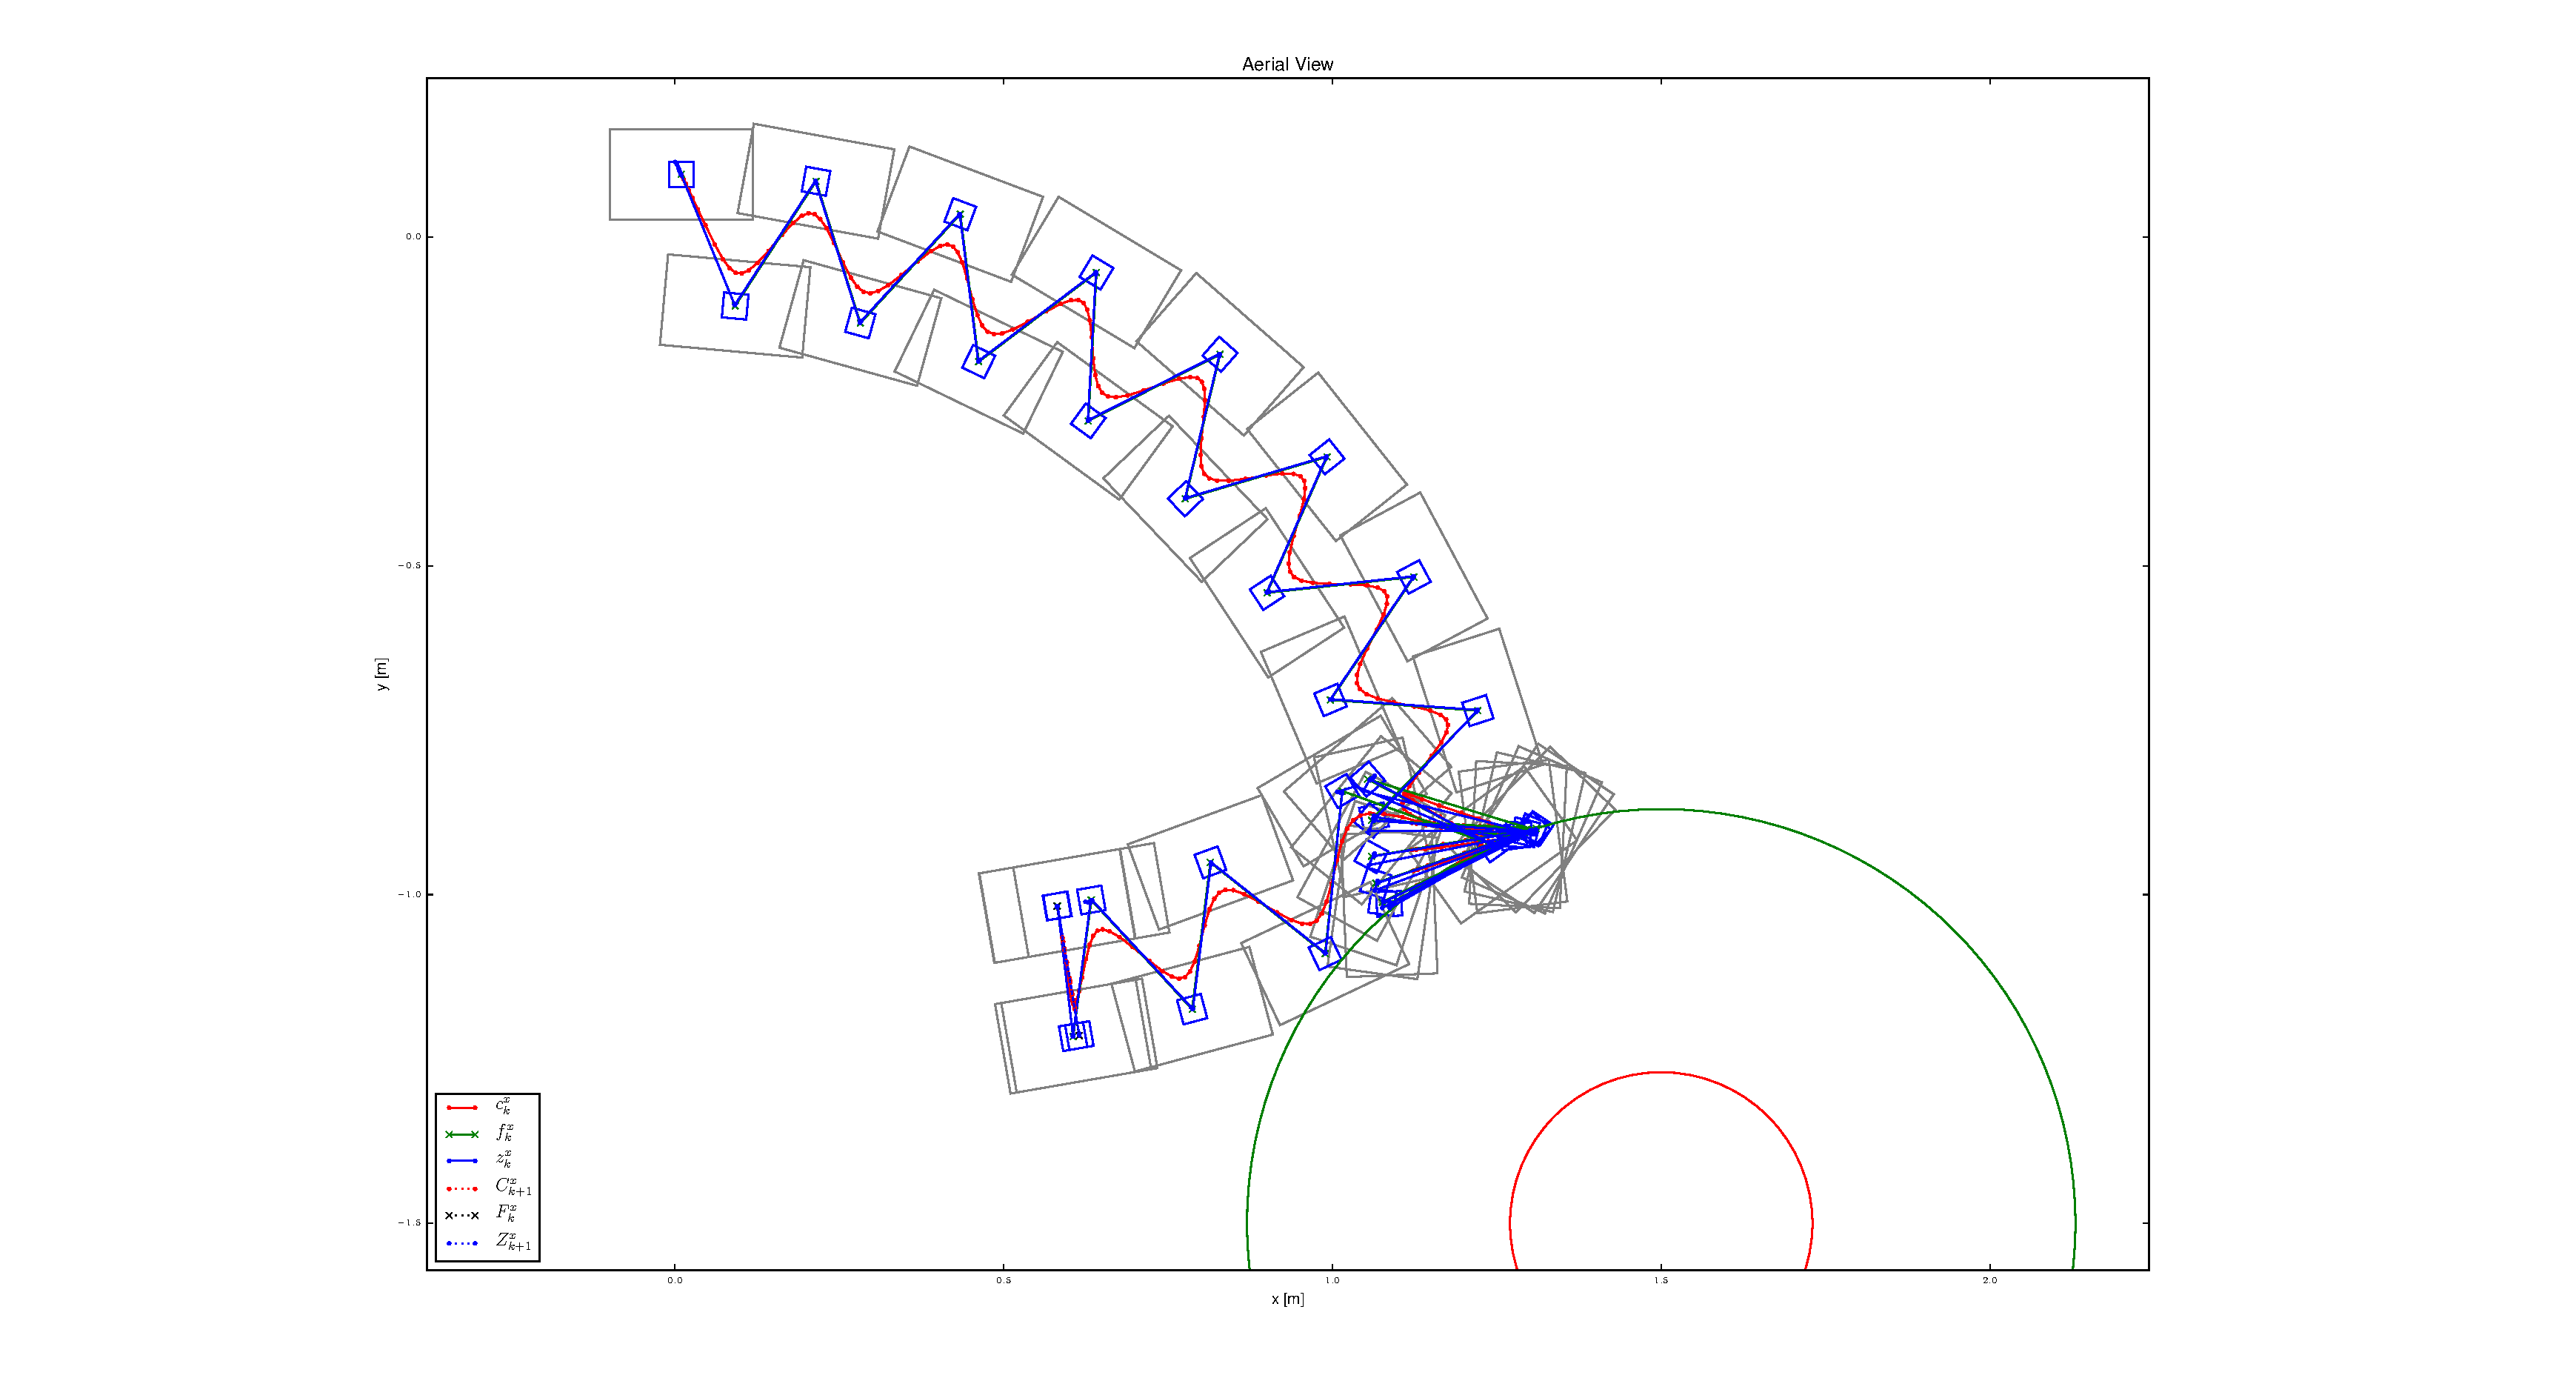
\includegraphics[trim={13.0cm 3.0cm 18.0cm 2.0cm},
        clip, angle=0, width=0.45\linewidth]{./setupB.pdf}}
        %trim={<left> <lower> <right> <upper>}
      \label{subfig:trajectoriesA}
    }
  \caption[Test cases \emph{A} and \emph{B}]
  {
  Center-of-mass and center-of-pressure trajectories
  for obstacle avoidance and foot-step orientation using NMPC.
  Situation~\emph{A} : Constant forward velocity.
  Situation~\emph{B} : Constant forward and angular velocity.
  }
  \label{fig:trajectories}
  \end{center}
\end{figure}

The setup \emph{B}, depicted in Fig.~\ref{fig:hrp2_experiment} and \ref{fig:trajectories} is quite similar.
A constant velocity ${Vel}_{k+1}^{ref}=[0.2,0,0.2]$ including rotation around the vertical axis is sent to the walking pattern generator.
The robot starts to describe a circle and get stuck in front of the obstacle.
As the constraint is locally linearized, and because the reference velocity in translation is going towards the constraint,
the robot is blocked in translation.
Thus, it stops moving forward and continues to turn on spot, as the angular velocity is not conflicting with the constraint.
Once the robot has passed the obstacle, it can freely move forward and describe a circle again.

\subsection{Robustness to perturbation}
%
%A disturbance test case has been performed in simulation.
%A force has been introduced in the feedback of the pattern generator as an additional CoM acceleration.
%The maximum range of lateral force that can be handled is $[-45 ; 90]\,N$.
%The asymmetrical aspect comes from the fact that the robot is walking on spot at the moment of the push so the CoM has already a lateral velocity and acceleration.
%In addition the kinematic constraints are not symmetrical as one leg is already in the air.
%The maximum range of forward and backward perturbation is $[-115 ; 115]\,N$ as the problem here is symmetrical.
%Above these force limits the QPs become infeasible.
%A way to avoid this problem is to bound the input force.






%\addtolength{\textheight}{-2cm}







A disturbance test case has been performed in simulation.
The disturbance is introduced as a force added to the CoM acceleration in the walking pattern generator.
This force is applied during $100\,ms$.
Two kind of disturbances were considered: on the sagittal plane (both directions) and on the coronal plane (both directions).
In both cases, we considered two walking situations: forward and on spot.

On the coronal plane, the maximum lateral force that can be handled is $90\,N$, equivalent to $-0.63\,J$, and $-45\,N$, equivalent to $0.675\,J$.
The asymmetry comes from the fact that the robot might be in a different walking situation during the push.
The push may occur when the robot can perform a step without collision, or when it cannot.
In the latter case, the magnitude of the force that can be rejected is smaller.
We found roughly the same values for the two walking situations.

When walking on spot, the maximum forward and backward perturbation is $\pm 115\,N$ ,equivalent to $\pm 0.86\,J$, as the problem  is symmetrical.
When walking forward, the maximum disturbance is smaller in the forward direction.
The interval found is $[-160;70]\,N$, equivalent to $[-1.12;1.54]\,J$.
%\end{itemize}


\subsection{Computation time}

This algorithm runs online on the \mbox{HRP-2} CPU board ($Intel(R) \, Core2(TM) \, Duo \, E7500$, one core used, $2.8 \, GHz$, $3 \, Mb$ of cache size, on Ubuntu 10.04 LTS).
So only counts the iteration when the NMPC is computed.
Thus the statistics apply only when the walking pattern generator is computed.
The time measurement has been performed on the complete control architecture (see Fig.~\ref{fig:combined_feedback_scheme}).
\begin{center}
\begin{tabular}{|c|c|c|}
  \hline
  \emph{Time consumption}  & experiment A & experiment B \\
  \hline
    Average ($ms$)            & $3.95$ & $4.00$ \\
  \hline
    Standard deviation ($ms$) & $0.14$ & $0.18$ \\
  \hline
    Minimum ($ms$)            & $3.34$ & $3.085$ \\
  \hline
    Maximum ($ms$)            & $4.34$ & $5.19$ \\
  \hline
\end{tabular}
\end{center}
The robot is controlled at a period of $5 \, ms $.
Over all the experiences, there was only one iteration over $5 \, ms $. It is due to the stabilizer which consumes more CPU time when the robot is in a configuration leading to a kinematic singularity.
The algorithm is still computed every $100\,ms$ to simplify the double support phase handling.

\subsection{Cost function gains}

%\begin{center}
%\begin{tabular}{|c|c|c|}
%  \hline
%  $\alpha$ & $\beta$ & $\gamma$ \\
%  \hline
%  $5$ & $10^3$ & $5\;10^{-3}$ \\
%  \hline
%\end{tabular}
%\end{center}
The cost function gains are : $\alpha=2.5$, $\beta=10^3$ and $\gamma=10^{-5}$.
As specified in Sec.~\ref{SubSec:costFunction}, $\alpha$ is the reference tracking gain, $\beta$ is a gain maintaining the CoP close to the center of the foot, and $\gamma$ is the regularization gain.
They were chosen according to their experimental performance.
The chosen cost function gives different foot steps compared to \cite{deits:ichr:14}.
Where the minimization of a cost-to-go criteria as in \cite{deits:ichr:14} was used, here the robot follows a velocity prescribed by the user and can differ from it locally to avoid an obstacle.
This local method runs in real time at a lower level of control which copes with potential evolution of the environment after a first planning.

\subsection{qpOASES solver}

The nonlinear problem is linearized analytically (see Sec.~\ref{sec:linearization}) to form a quadratic problem with linear constraints.
The off-the-shelf solver qpOases \cite{Ferreau2014} is used to solve the respective QP.
This solver is a primal solver implementing an online active set strategy.

\section{Conclusion}

In this chapter we presented a real-time embedded nonlinear walking pattern generator.
Nonlinear inequalities make possible to choose the foot step automatically while considering orientation
and local avoidance of convex obstacles.
Its performance was demonstrated in two different experiments using the humanoid robot \mbox{HRP-2}.
The computational cost of the walking pattern generator is $2 \,ms$ on the robot.
An extension to our method would be to use a planner in addition to the walking pattern generator.